\chapter{Quantum Noise}
\lecture{18}{18 Nov. 10:30}{}  % L17이랑 통합
\section{Introduction}
지금까지 우리는 quantum computer가 사용하는 system이 "완벽하다"고 가정하였다. (i.e., 외부 환경과 완벽히 독립된 닫힌 계)
하지만 실제로는 외부 환경과 상호작용하면서 \textit{noise}가 발생한다. 따라서 이번 챕터에서는 \textit{open system}에서의 quantum dynamics를 정의하고 이를 사용하여 noise를 나타내고 분석하는 방법을 다루고자한다. 

\section{Axiomatic approach to quantum evolutions}
Open system에서의 quantum evolution을 정의하기 위하여, 먼저 몇 가지 notation을 정의하고자한다.
\begin{itemize}[itemsep=0.05cm]
    \item $\mathcal{D}(\mathcal{H})$ : Hilbert space $\mathcal{H}$에 작용하는 density operator (density matrix)들의 집합
    \item $\mathcal{L}\left(\mathcal{H}_A, \mathcal{H}_B\right)$ : Hilbert space $\mathcal{H}_A$에서 Hilbert space $\mathcal{H}_B$로 가는 linear operator들의 space\footnote{ $\mathcal{L}(\mathcal{H})$ : 자기 자신(Hilbert space $\mathcal{H}$)으로 가는 square linear operator들의 spaces}
\end{itemize}
위의 표현을 이용하면, general quantum operation $\mathcal E : \mathcal D(\mathcal H_A) \rightarrow \mathcal D(\mathcal H_B)$을 나타낼 수 있다. ($\mathcal E(\rho_A) \in \mathcal D(\mathcal H_B)$ if $\rho_A \in \mathcal D(\mathcal H_A)$는 general quantum operation을 나타낸다.\footnote{operator가 작용하기 전과 후, Hilbert space가 같지 않아도 된다는 것에 유의하라.})

\vspace{0.6em}

이제 quantum operation; channel이 \textbf{convex linear}이라고 가정하자.($\lambda \in[0,1]$ and $\rho_A, \sigma_A \in \mathcal{D}\left(\mathcal{H}_A\right)$)
\begin{equation}
    \mathcal{E}\left(\lambda \rho_A+(1-\lambda) \sigma_A\right)=\lambda \mathcal{E}\left(\rho_A\right)+(1-\lambda) \mathcal{E}\left(\sigma_A\right)\label{eq:convex-evolution}
\end{equation}

Quantum operation $\mathcal E$가 convex linear 라는 것은 \textit{ensemble}로 해석할 수 있다. 에를 들어, 어떤 동전을 던져서 그 결과에 따라 $\rho_A$, $\sigma_A$ 두 상태중에서 하나의 상태로 준비한 뒤 quantum operation $\mathcal E$를 적용하는 상황을 가정하자. 만약 두 주어진 상태가 $\rho_A, \sigma_A$ 중에서 무엇인지 알지 못하는 상황이라면, mixed state에 operation을 가한 상황으로 해석되기 때문에 이는 Eq.~\eqref{eq:convex-evolution}의 좌변에 해당된다. 반대로, 두 주어진 상태가 $\rho_A, \sigma_A$ 중에서 무엇인지 알고 있다면, 이는 Eq.~\eqref{eq:convex-evolution}의 우변에 해당될 것이다.
\vspace{0.6em}

이제 quantum channel의 정의역과 공역을 density operator만이 아닌 모든 linear operator에 대해서 확장하자. 이때 quantum channel이 \textit{convex linearity를 만족하기 위한 조건}은 다음과 같다.
\begin{enumerate}
    \item A quantum channel $\mathcal E$ is a linear map
    \begin{equation}
        \mathcal{E}\left(\alpha X_A+\beta Y_A\right)=\alpha \mathcal{E}\left(X_A\right)+\beta \mathcal{E}\left(Y_A\right)
    \end{equation}
    \item A quantum channel $\mathcal E$ is positive map : Density operator는 반드시 density operator로 사상되어야 하므로 연산 전 후 \textbf{positivity}를 보존해야 한다.
    \begin{definition}[Positive map]
        만약 모든 positive semi-definite $X_A \in \mathcal{L}\left(\mathcal{H}_A\right)$에 대해서, 사상 결과 $\mathcal{M}\left(X_A\right)$가 positive semi-definite 이라면 $\mathcal{M}: \mathcal{L}\left(\mathcal{H}_A\right) \rightarrow \mathcal{L}\left(\mathcal{H}_B\right)$ 은 positive map이다. 
    \end{definition}
    \item A quantum channel $\mathcal E$ is \textit{completely} positive map : 위의 조건에 더해, composite system과 entanglement를 고려해도 여전히 positivity를 유지하기 위해서 completely positive map의 조건으로 확장된다. 
    예를 들어, composite system $\rho_{RA} \in \mathcal D(\mathcal H_R \otimes \mathcal H_A)$에 대해서 quantum channel을 오직 system $A$에만 가하더라도 (i.e., $I_R \otimes \mathcal E_A$) 전체 composite system의 positivity를 보존해야 한다.\\
    수학적으로, $\{\ket i_R\}$를 $\mathcal H_R$의 orthonormal basis라고 하자. 이때 모든 operator $X_{RA} \in \mathcal L(\mathcal H_R \otimes \mathcal H_A)$는 다음과 같이 표현할 수 있다.
    \begin{equation*}
        X_{RA} = \sum_{i,j} \ket i \bra j_R \otimes X_A^{i,j}
    \end{equation*}
    이때 $\mathcal I_R \otimes \mathcal E_{A\rightarrow B}$의 작용은 다음과 같이 표현된다.
    \begin{align*}
        \left(\mathcal I_R \otimes \mathcal E_{A\rightarrow B}\right)\left(X_{R A}\right) &= \left(\mathcal I_R \otimes \mathcal E_{A\rightarrow B}\right)\left(\sum_{i,j} \ket i \bra j_R \otimes X_A^{i,j}\right) \\
        &= \sum_{i,j} \ket i \bra j_R \otimes \mathcal E_{A\rightarrow B}\left(X_A^{i, j}\right)
    \end{align*}
    즉, local operation은 reference system $R$에 대해서는 아무런 효과를 주지 않는다.
    \begin{definition}[Completely positive map]
        만약, 어떤 arbitrary size의 reference system $R$에 대해서도 $\mathcal{I}_R \otimes \mathcal{M}$이 positive map이라면, $\mathcal{M}$은 completely positive map이다.
    \end{definition}
    \item A quantum channel $\mathcal E$ is \textit{trace-preserving} : density operator는 그대로 density operator로 사상되어야 하므로 trace를 보존해야한다. 이를 linear operator로 확장하면 모든 linear operator에 대해 trace를 보존해야한다.
    \begin{equation*}
        \text{Tr}\left(\mathcal E\left(X_A\right)\right) = \text{Tr}\left(X_A\right)
    \end{equation*}
\end{enumerate}

따라서 정리하자면, \textit{Quantum channel}은 다음을 만족해야한다. 
\begin{definition}
    A quantum channel is a \textit{linear, completely positive, trace preserving map}.
\end{definition}

\vspace{0.6em}

위의 3가지 조건을 일일이 확인하지 않고도 쉽게 확인할 수 있는 방법이 있다. 다음 Theorem에 따르면, 3가지 조건을 모두 만족하는 map은 Choi-Kraus decomposition이 가능하며, Choi-Kraus decomposition을 가지는 map은 3가지 조건을 모두 만족한다.
\begin{theorem}[Choi-Kraus]\label{thm:Choi-Kraus}
    A map $\mathcal{E}: \mathcal{L}\left(\mathcal{H}_A\right) \rightarrow \mathcal{L}\left(\mathcal{H}_B\right)$ is linear, completely positive, and tracepreserving \textit{if and only if} it has a Choi-Kraus decomposition:
    $$ \mathcal{E}_{A \rightarrow B}\left(X_A\right)=\sum_{l=0}^{d-1} V_l X_A V_l^{\dagger}, $$
    where $X_A \in \mathcal{L}\left(\mathcal{H}_A\right), V_l \in \mathcal{L}\left(\mathcal{H}_B, \mathcal{H}_A\right)$ for all $l \in\{0, \ldots, d-1\}$,
    and the Kraus operator satisfy the completeness relation and $d \le \text{dim}\left(\mathcal{H}_A\right) \times \text{dim}\left(\mathcal{H}_B\right)$.
    $$\sum_{l=0}^{d-1} V_l V_l^{\dagger}=I_A$$
\end{theorem}
\textit{Proof. See Appendix A.} $\Box$

\begin{figure}[h]
    \centering
    \vspace{0.5em}
    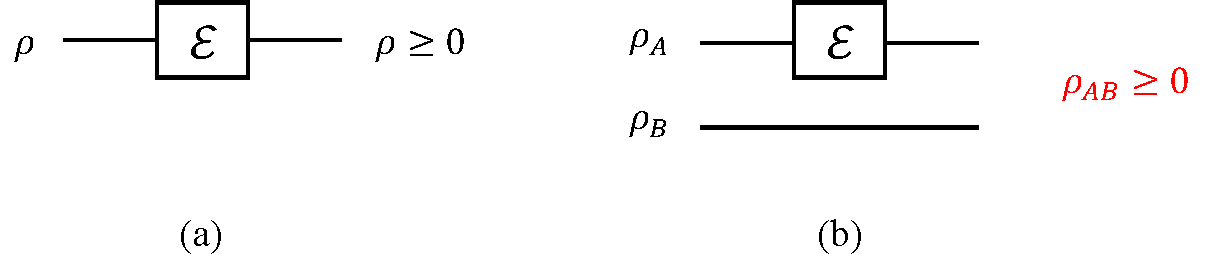
\includegraphics[width=0.75\textwidth]{figures/positive.pdf}
    \caption{(a) positive map, (b) completely positive map}
    \label{fig:positive}
\end{figure}

\section{Interpretation of quantum channels}
이번 섹션에서는 \textit{Quantum channel}의 두 가지 해석을 다루고자한다.
\subsection{Noisy evolution as the loss of a measurement outcome}
어떤 System이 density operator $\rho$로 표현되고 measurement set $\{ M_k \}$를 사용하여 측정을 수행한다고 하자. ($\sum_k M_k^\dagger M_k = I$) 이때, outcome $k$를 얻을 확률은 \textit{잘 알다시피} 다음과 같고
\begin{equation*}
    p(k)=\operatorname{Tr}\left[M_k^{\dagger} M_k \rho\right]
\end{equation*}
post-measurement state는 다음과 같다. 
\begin{equation*}
    \frac{M_k \rho M_k^{\dagger}}{p(k)}
\end{equation*}

그런데 만약 우리가 측정해서 얻은 \textbf{outcome이 무엇인지 알지 못한다면} post-measurement state는 가능한 모든 outcome들에 대해 \textit{mixed state}로 표현된다. Ensemble description으로 표현하면 다음과 같고
\begin{equation*}
    \bigg\{p(k), \frac{M_k \rho M_k^{\dagger}}{p(k)}\bigg\}
\end{equation*}
이는 다음과 같은 density matrix로 표현된다. 
\begin{equation*}
    \sum_k \cancel{p(k)} \frac{M_k \rho M_k^{\dagger}}{\cancel{p(k)}}=\sum_k M_k \rho M_k^{\dagger}
\end{equation*}
위 수식에서처럼 mixed state의 density matrix는 \hyperref[thm:Choi-Kraus]{Choi-Kraus decomposition} 표현과 동일하다. 따라서 quantum channel을 measurement를 수행하고 outcome을 확인하지 않는 연산으로 생각할 수 있다. 


\subsection{Noisy evolution from a unitary interaction}
Quantum channel을 해석하는 또 다른 방법은 environment가 unitary interaction을 통해 우리의 system에 영향을 주는 상황으로 이해하는 것이다. Quantum system $A$는 state $\rho_A$로, environment system $E$는 pure state $\ket{0}_E$로 초기화되었다고 하자.\footnote{Environment를 pure state로 표현할 수 있는 이유는, environment가 pure state가 아니더라도 얼마든지 reference system을 추가하여 purification을 적용하면 pure state로 표현할 수 있기 때문이다.} 
전체 system에 대해 joint time evolution, $U_{AE}$이 발생하면 우리는 environment system $E$에 대한 접근 권한이 없기 때문에, partial trace를 취한 system $A$에 대한 상태만을 얻을 수 있다. 
\begin{equation*}
    \sigma_A=\operatorname{Tr}_E\left[U_{A E}\left(\rho_A \otimes|0\rangle\langle 0|\right) U_{A E}^{\dagger}\right]
\end{equation*}
이 상태를 정리하면, Kraus representation을 얻을 수 있다.\todo{step 2 understand} ($B_i \triangleq \langle i_E | U_{AE} | 0_E \rangle$)
\begin{equation*}
    \operatorname{Tr}_E\left[U_{A E}\left(\rho_A \otimes|0\rangle\langle 0|\right) U_{A E}^{\dagger}\right] = \sum_i \langle i|_E U_{AE} (\rho_A \otimes \ket 0 \bra 0) U^{\dagger}_{AE} \ket i_{E} = \sum_i B_i \rho_A B_i^\dagger
\end{equation*}
$B_i$가 completeness relation을 만족하는지 쉽게 확인할 수 있다.
\begin{align*}
    \sum_i B_i^{\dagger} B_i &= \sum_i\langle i|_E U_{A E} | 0\rangle_E^{\dagger}\langle i|_E U_{A E} | 0\rangle_E = \sum_i\langle 0|_E U_{A E}^{\dagger} | i\rangle_E\langle i|_E U_{A E} | 0\rangle_E 
    \\ &= \langle 0|_E U_{A E}^{\dagger} \sum_i | i\rangle_E\langle i|_E U_{A E} | 0\rangle_E =\langle 0|_E U_{A E}^{\dagger} U_{A E} | 0\rangle_E = I_A .
\end{align*}

반면, Kraus operator가 noisy evolution을 나타낸다는 사실도 쉽게 확인할 수 있다. Kraus operator $\{E_k\}$, $\sum_k E_k^\dagger E_k = I_A$에 대해 $\{\ket{e_k}\}$를 각각 $E_k$에 대응되는 orthogonal basis set이라고 하자. 
$\ket \psi \ket{e_0}$에 대해서 다음과 같이 동작하는 operator $U$를 정의하자.\footnote{$\ket{e_0}$는 environment의 임의의 standard state이다.}
\begin{equation*}
    U|\psi\rangle\left|e_0\right\rangle \equiv \sum_k E_k|\psi\rangle\left|e_k\right\rangle,
\end{equation*}
$U$는 다음과 같이 composite system에 대해 norm을 보존한다. (by completeness relation of Kraus operator)
\begin{equation*}
    \left.\langle\psi| e_0\left|U^{\dagger} U\right| \varphi\right\rangle\left|e_0\right\rangle=\sum_k\langle\psi| E_k^{\dagger} E_k|\varphi\rangle=\langle\psi | \varphi\rangle,
\end{equation*}
따라서, operator $U$는 전체 composite system에 대해서 동작하는 unitary operator로 생각할 수 있다.
\begin{equation*}
    \operatorname{Tr}_E\left[U\left(\rho \otimes\left|e_0\right\rangle\left\langle e_0\right|\right) U^{\dagger}\right]=\sum_k E_k \rho E_k^{\dagger} .
\end{equation*}

\subsection{Freedom in the operator-sum representation}
지금까지 우리는 operator-sum representation을 사용하여 general quantum channel을 표현할 수 있다는 것을 확인하였다. 그렇다면, 과연 \textit{Choi-Kraus decomposition}은 unique한 표현인가?

이를 확인하기 위해서, single qubit에 작용하는 2가지 channel $\mathcal E, \mathcal F$를 가정하자. 각 channel은 다음과 같은 Kraus operator $\{E_1, E_2\}$, $\{F_1, F_2\}$를 각각 가진다.
\begin{equation*}
    E_1=\frac{I}{\sqrt{2}}, \quad E_2=\frac{Z}{\sqrt{2}}, \quad F_1=|0\rangle\langle 0|, \quad F_2=|1\rangle\langle 1| .
\end{equation*}
놀랍게도 두 channel은 동일하다!
\begin{equation*}
    \mathcal{F}(\rho)=\frac{1}{2}\left[(E_1+E_2) \rho(E_1^{\dagger}+E_2^{\dagger})+(E_1-E_2) \rho(E_1^{\dagger}-E_2^{\dagger})\right ]= E_1 \rho E_1^{\dagger}+E_2 \rho E_2^{\dagger}=\mathcal{E}(\rho) .
\end{equation*}
이처럼 동일한 두 channel을 표현하는 서로다른 Kraus operator가 존재하는 반례를 찾았으므로 Choi-Kraus decomposition은 unique하지 않다. Operator-sum representation은 다음 정리를 따른다.
\begin{theorem}
    $\left\{E_i\right\}_{i=1}^m$와 $\left\{F_i\right\}_{i=1}^n$를 각각 $\mathcal{E}$와 $\mathcal{F}$에 대한 operation elements라고 하자. 두 집합 중에서 더 크기가 작은 집합에 zero operator를 추가하여, 두 집합의 크기가 동일하도록 만들 수 있다. 이때 $E_i = \sum_j u_{i j} F_j$가 되도록하는 complex number $u_{ij}$가 존재하면, $\mathcal{E}=\mathcal{F}$이다.
\end{theorem}


\section{Examples}
\subsection{Bit flip and phase flip channels}
\textit{Bit flip} channel은 $1-p$의 확률로 $X$ gate를 가하는 channel로, 다음의 operation elements를 가진다.
$$
E_0=\sqrt{p} I=\sqrt{p}\left(\begin{array}{ll}
1 & 0 \\
0 & 1
\end{array}\right), \quad E_1=\sqrt{1-p} X=\sqrt{1-p}\left(\begin{array}{ll}
0 & 1 \\
1 & 0
\end{array}\right) .
$$
Kraus operator들을 이용하면 bit flip channel이 다음과 같이 동작함을 알 수 있다.
\begin{equation*}
    \mathcal{E}(\rho) = E_0 \rho E_0^\dagger + E_1 \rho E_1^\dagger = p \cdot \rho + (1-p) \cdot X \rho X^\dagger
\end{equation*}

\textit{Phase flip} channel은 $1-p$의 확률로 $Z$ gate를 가하는 channel로, 다음의 operation elements를 가진다.
$$
E_0=\sqrt{p} I=\sqrt{p}\left(\begin{array}{ll}
1 & 0 \\
0 & 1
\end{array}\right), \quad E_1=\sqrt{1-p} Z=\sqrt{1-p}\left(\begin{array}{cc}
1 & 0 \\
0 & -1
\end{array}\right) .
$$
Phase flip channel은 \textit{dephasing}이라고도 불리는데, 이는 output state를 다음과 같이 표현할 수 있기 때문이다. 만약 $p = 1/2$라면, output state는 대각성분만 남게된다.
$$
p\left(\begin{array}{cc}
\rho_{00} & \rho_{01} \\
\rho_{10} & \rho_{11}
\end{array}\right)+(1-p)\left(\begin{array}{cc}
\rho_{00} & -\rho_{01} \\
-\rho_{10} & \rho_{11}
\end{array}\right)=\left(\begin{array}{cc}
\rho_{00} & (2 p-1) \rho_{01} \\
(2 p-1) \rho_{10} & \rho_{11}
\end{array}\right) .
$$


\textit{Bit-phase flip} channel은 $1-p$의 확률로 $Y$ gate를 가하는 channel이다.
$$
E_0=\sqrt{p} I=\sqrt{p}\left(\begin{array}{ll}
1 & 0 \\
0 & 1
\end{array}\right), \quad E_1=\sqrt{1-p} Y=\sqrt{1-p}\left(\begin{array}{cc}
0 & -i \\
i & 0
\end{array}\right) .
$$

\begin{figure}
    \centering
    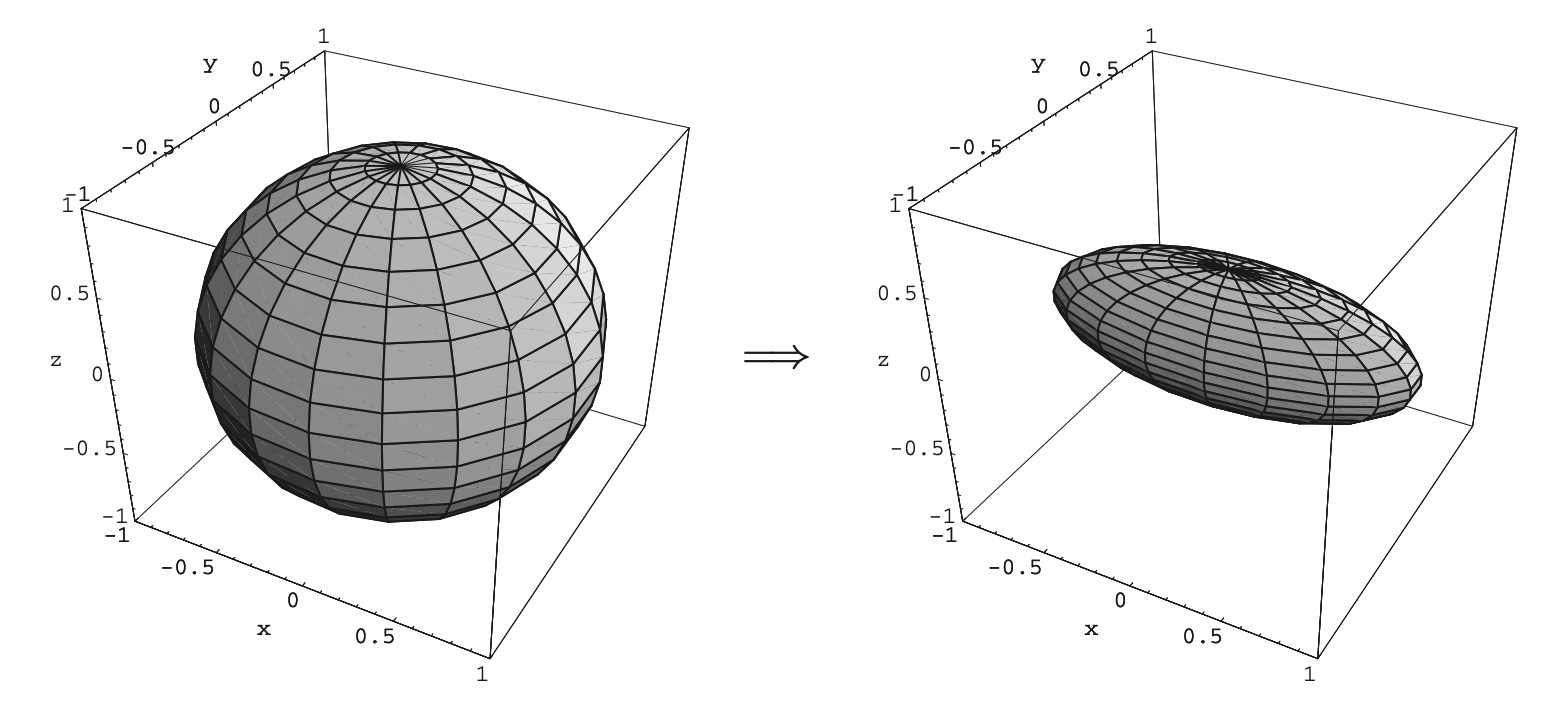
\includegraphics[width=0.55\textwidth]{figures/bit_flip.png}
    \caption{Bit flip channel \cite{nielsen2001quantum}}
    \label{fig:bit-flip}
\end{figure}

\subsection{Depolarizing channel}
\textit{Depolarizing} channel은 $p$의 확률로 \textbf{completely mixed state} $I/2$가 되는 channel으로, $I/2$는 기존 state에 대해 아무런 정보도 제공해주지 않기 때문에 quantum noise에서 매우 중요하게 다뤄지는 noise type이다.
Chanel을 통과한 후 state는 다음과 같이 표현된다.
\begin{equation*}
    \mathcal{E}(\rho)=\frac{p I}{2}+(1-p) \rho
\end{equation*}
다음의 관계를 이용하면,
\begin{equation*}
    I=\frac{1}{2}(\rho+X \rho X+Y \rho Y+Z \rho Z)
\end{equation*}
다음과 같이 operator-sum representation으로 나타낼 수 있다. 
\begin{equation*}
    \mathcal{E}(\rho)=\left(1-\frac{3 p}{4}\right) \rho+\frac{p}{4}(X \rho X+Y \rho Y+Z \rho Z) 
\end{equation*}
확률을 더 간단하게 표현하기 위해 다음과 같이 나타내기도 한다.
\begin{equation*}
    \mathcal{E}(\rho)=\left(1-p\right) \rho+\frac{p}{3}(X \rho X+Y \rho Y+Z \rho Z)
\end{equation*}

\subsection{Amplitude damping channel}
마지막으로 소개할 noise는 \textit{physical noise}의 개념에 더 가깝다.\footnote{앞서 소개한 noise들은 $I$ operator에 대해서 여전히 $I$로 동작함을 보장하지만 이 noise는 이를 보장하지 않는다.} High energy state인 $\ket 1 \bra 1$에서 점점 energy가 감소하먼서 $\ket 0 \bra 0$으로 상태가 변화하는 noise이다. 
\begin{equation*}
    \mathcal{E}(\rho)=E_0 \rho E_0^{\dagger}+E_1 \rho E_1^{\dagger}
\end{equation*}
Operation elements는 각각 다음과 같다.
\begin{equation*}
    E_0=\left(\begin{array}{cc}
        1 & 0 \\
        0 & \sqrt{1-\gamma}
        \end{array}\right), \quad E_1=\left(\begin{array}{cc}
        0 & \sqrt{\gamma} \\
        0 & 0
        \end{array}\right) .
\end{equation*}
즉, $E_1$은 $\ket 1$ state를 $\ket 0$ state로 변화시키며 $E_2$는 $\ket 0$ state의 amplitude를 감쇠시킨다. 따라서 이 channel을 사용하면 $\ket 0$ state는 항상 그대로 유지되지만 $\ket 1$ state에 대한 amplitude는 점차 감쇠되게 된다.